\documentclass[../thesis.tex]{subfiles}

\begin{document}

\section{Công nghệ di động}
	
	Với tính tiện lợi và tích hợp nhiều chức năng hữu ích, Smartphone hiện nay được sử dụng khá rộng rãi và phổ biến trên toàn thế giới, trở thành một phần cuộc sống của không ít người. Ngoài vai trò là một chiếc điện thoại nghe gọi bình thường, Smartphone còn có nhiều chức năng khác rất hữu ích như chụp ảnh, quay video, tích hợp GPS, cung cấp tùy biến cho hệ điều hành, đặc biệt trong số đó là kho ứng dụng với vô vàn chức năng khác nhau phục vụ từ những nhu cầu cá nhân cho tới những yêu cầu cấp thiết trong công việc, có thể kể đến như Ứng dụng mạng xã hội Facebook, Twitter, ứng dụng mua sắm Shopify, ứng dụng trình duyệt Web Chrome, ứng dụng bản đồ Google Maps ...
	
	\begin{figure}[ht!]
		\centering
		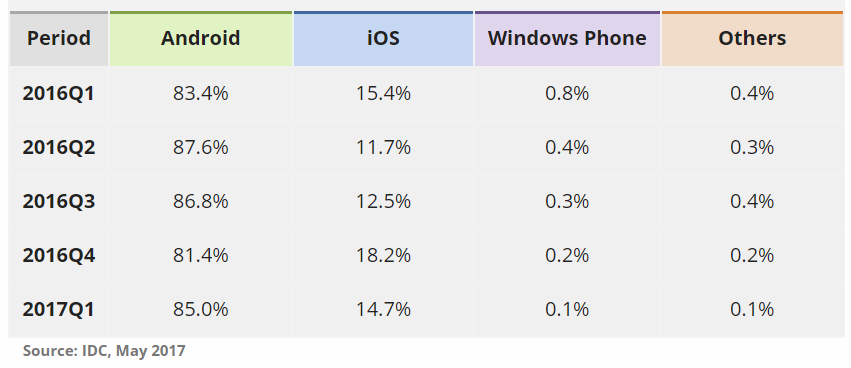
\includegraphics[width=1\textwidth]{thiphansmartphone.png}
		\caption{Thống kê thị phần Smartphone OS, quí I năm 2017}
		\cite{android:thongke_thiphansmartphone}
		\label{fig:thongke_thiphan}
	\end{figure}
	
	Các Smartphone được xem như là những chiếc máy tỉnh bỏ túi, được chạy bởi một hệ điều hành riêng, quản lý và tùy chỉnh bởi người dùng. Android của Google và iOS của Apple hiện tại là 2 hệ điều hành Smartphone phổ biến nhất thế giới, theo thống kê vào Quí I năm 2017, 2 hệ điều hành chiếm thị phần 99,8\% của các Smartphone trên toàn thế giới.
	
	Với khoảng 2,53 tỷ thiết bị đang hoạt động trên toàn thế giới\cite{android:thongke_ngdungsmartphone}, công nghệ Smartphone được xem như là một xu hướng phát triển mạnh mẽ của ngành Công nghệ thông tin trong những năm tới.
	
	\subsection{Hệ điều hành Android}
	"Android là một hệ điều hành dựa trên nền tảng Linux được thiết kế dành cho các thiết bị di động có màn hình cảm ứng như điện thoại thông minh và máy tính bảng. Ban đầu, Android được phát triển bởi Tổng công ty Android, với sự hỗ trợ tài chính từ Google và sau này được chính Google mua lại vào năm 2005.Chiếc điện thoại đầu tiên chạy Android được bán vào năm 2008. Android có một cộng đồng lập trình viên đông đảo chuyên viết các ứng dụng để mở rộng chức năng của thiết bị, bằng một loại ngôn ngữ lập trình Java có sửa đổi. Vào tháng 10 năm 2012, có khoảng 700.000 ứng dụng trên Android, và số lượt tải ứng dụng từ Google Play, cửa hàng ứng dụng chính của Android, ước tính khoảng 25 tỷ lượt. Android chiếm 87,7\% thị phần điện thoại thông minh trên toàn thế giới vào thời điểm quý 2 năm 2017, với tổng cộng 2 tỷ thiết bị đã được kích hoạt và 1,3 triệu lượt kích hoạt mỗi ngày."\cite{wiki:android}
	
	Các ưu điểm khi phát triển một ứng dụng Android:
	\begin{itemize}
		\item \textbf{Mã nguồn mở:} Android cung cấp một platform mã nguồn mở, đồng nghĩa với việc sử dụng bộ công cụ phát triển cho Android (hay Android Software Development KIT - Android SDK) là hoàn toàn miễn phí. Các nhà phát triển ứng dụng không cần phải lo lắng về vấn đề bản quyền hay giá cả. Đồng thời, với thị phần đông đảo trong thị trường Smartphone, các nhà phát triển có thể sở hữu một thiết bị chạy Android với giá khá rẻ để phục vụ cho việc xây dựng ứng dụng. Ngoài ra, là mã nguồn mở, cũng đồng nghĩa với việc cộng đồng phát triển Android cũng sẽ đông hơn, qua đó các nhà phát triển có thể chia sẻ, giải quyết các khó khăn thắc mắc cùng với nhau. Những điều trên tạo nên một môi trường lý tưởng cho việc phát triển một ứng dụng điện thoại hiệu quả và nhanh chóng.
		
		\item \textbf{Công cụ mạnh mẽ:} Android Studio ra đời vào năm 2013, bây giờ được xem như là công cụ phát triển ứng dụng Android phổ biến nhất với \textcolor{red}{...} người dùng. Sử dụng Java là một trong những ngôn ngữ lập trình phổ biến nhất trên thế giới, là ngôn ngữ chính, giúp cho việc tiếp cận và làm quen cũng như học hỏi diễn ra dễ dàng hơn, đồng thời mang lại lợi ích của việc sử dụng các thư viện hữu ích đã có sẵn trong cộng đồng lập trình Java. Ngoài ra, Android Studio còn tích hợp các bộ xây dựng sẵn giúp cho việc Debug hay tung ra sản phẩm diễn ra được dễ dàng hơn.
		
		\item \textbf{Giao diện dễ tùy biến: } Giao diện là một phần rất quan trọng trong việc đánh giá ứng dụng. Với bộ công cụ của mình, Android cung cấp cho những nhà phát triển khả năng tùy biến giao diện rất dễ dàng. Cụ thể, với khoảng 50 thành phần cơ bản (Button, Form, TextView, ...) trong bộ công cụ phát triển cùng với một số các thư viện hỗ trợ được cung cấp khác như Design, RecyclerView, ...
		\begin{figure}[ht!]
			\centering
			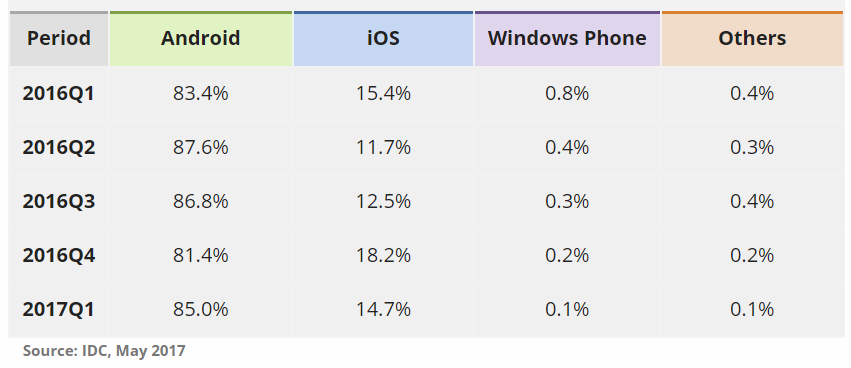
\includegraphics[width=1\textwidth]{thiphansmartphone.png}
			\caption{Giao diện Android}
			\label{fig:minhhoa_giaodien}
		\end{figure}
		\item \textbf{Tài liệu rõ ràng: } Cùng với bộ công cụ của mình, tài liệu cho việc học và sử dụng công cụ cũng được Google luôn luôn cập nhật nhanh chóng và đầy đủ. Kể từ khi ra đời, Android hiện nay có 14 phiên bản, trong đó các phiên bản Lollipop (5.0), Marshmallow (6) và Nougat(7) hiện đang là những phiên bản phổ biến nhất, mỗi phiên bản có những khác nhau ảnh hưởng đến việc phát triển ứng dụng, song chúng đều được mô tả khá đầy đủ trong tài liệu hướng dẫn, giúp cho việc phát triển tính tương thích của ứng dụng diễn ra dễ dàng hơn.
	\end{itemize}

	\subsection{Phát triển ứng dụng trên Android}	
	\begin{figure}[ht!]
		\centering
		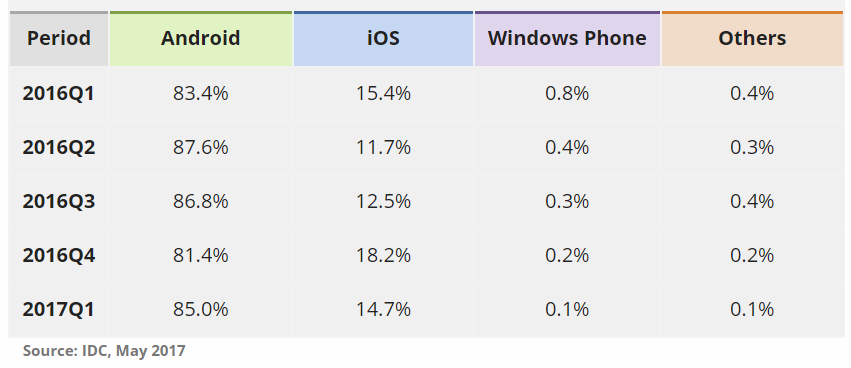
\includegraphics[width=1\textwidth]{thiphansmartphone.png}
		\caption{Minh họa android}
		\label{fig:minhhoa_android}
	\end{figure}	
	
	Với hơn 3,4 triệu ứng dụng trong Store của mình, Google Store hiện tại được xem như là kho ứng dụng điện thoại lớn nhất thế giới\cite{android:googlestore}. Đây được xem như là môi trường phát triển chính cho việc phát triển ứng dụng điện thoại trên Android.
	
	Như đã nhắc đến ở trên, Android Studio là phần mềm nhóm em sẽ sử dụng cho việc phát triển ứng dụng. 
	
	Một trong những chức năng khá hữu ích từ hệ điều hành Android chính là công nghệ GPS, theo thống kê năm 2014, 50\% người mua sắm qua Smartphone sử dụng GPS để tìm đường đi, 33\% chủ nhân của Smartphone chia sẻ địa điểm của họ với nhà bán lẻ qua việc đăng ký dịch vụ.\cite{android:thongke1}
	
	\subsection{title}

\section{Web API}

\end{document}